\documentclass[letter]{article}
\usepackage{enumerate}
\usepackage{amsmath}
\usepackage{amssymb}
\usepackage{amsfonts}
\usepackage{amsthm}
\usepackage{latexsym}
\usepackage{mathrsfs}
\usepackage{eufrak}
\usepackage[pdftex]{graphicx}
\usepackage{color}
\usepackage{mathrsfs}
\usepackage[x11names, rgb]{xcolor}
\usepackage[utf8]{inputenc}
\usepackage{tikz}
\usepackage{dot2texi}
\usetikzlibrary{snakes,arrows,shapes}
\setlength{\topmargin}{-0.5in} \setlength{\textwidth}{6.5in}
\setlength{\oddsidemargin}{0.0in} \setlength{\textheight}{9.1in}
\def\pdfshellescape{1}
\newlength{\pagewidth}
\setlength{\pagewidth}{6.5in} \pagestyle{empty}

\newcommand{\R}{\mathbb{R}}
\newcommand{\N}{\mathbb{N}}
\newcommand{\B}{\mathfrak{B}}
\newcommand{\Z}{\mathbb{Z}}
\newtheorem{theorem}{Theorem}[section]
\newtheorem{lemma}[theorem]{Lemma}
\newtheorem{proposition}[theorem]{Proposition}
\newtheorem{corollary}[theorem]{Corollary}

\newenvironment{definition}[1][Definition]{\begin{trivlist}
\item[\hskip \labelsep {\bfseries #1}]}{\end{trivlist}}
\newenvironment{example}[1][Example]{\begin{trivlist}
\item[\hskip \labelsep {\bfseries #1}]}{\end{trivlist}}
\newenvironment{remark}[1][Remark]{\begin{trivlist}
\item[\hskip \labelsep {\bfseries #1}]}{\end{trivlist}}

\title{CSE 350 Spring 2010 HW \#1}
\date{}
\author{Chao Xu}
\begin{document}
\maketitle
\vspace{-.5in}
\section*{1.4f}
$\{w|w$ has an odd number of \textbf{a}'s$\}$\\
\begin{tikzpicture}[>=latex',line join=bevel,]
  \pgfsetlinewidth{1bp}
%%
\pgfsetcolor{black}
  % Edge: q_b -> q_a
  \draw [->,>=stealth',shorten >=1pt] (203bp,16bp) .. controls (192bp,12bp) and (177bp,8bp)  .. (164bp,11bp) .. controls (160bp,12bp) and (156bp,13bp)  .. (143bp,18bp);
  \draw (173bp,22bp) node[right] {$a$};
  % Edge: start -> q_a
  \draw [->,>=stealth',shorten >=1pt] (54bp,31bp) .. controls (63bp,31bp) and (72bp,31bp)  .. (92bp,31bp);
  % Edge: q_b -> q_b
  \draw [->,>=stealth',shorten >=1pt] (221bp,61bp) .. controls (220bp,71bp) and (224bp,80bp)  .. (231bp,80bp) .. controls (235bp,80bp) and (239bp,76bp)  .. (241bp,61bp);
  \draw (231bp,89bp) node[right] {$b$};
  % Edge: q_a -> q_b
  \draw [->,>=stealth',shorten >=1pt] (146bp,31bp) .. controls (159bp,31bp) and (175bp,31bp)  .. (200bp,31bp);
  \draw (173bp,39bp) node[right] {$a$};
  % Edge: q_a -> q_a
  \draw [->,>=stealth',shorten >=1pt] (111bp,57bp) .. controls (110bp,67bp) and (113bp,76bp)  .. (119bp,76bp) .. controls (123bp,76bp) and (125bp,72bp)  .. (127bp,57bp);
  \draw (119bp,85bp) node[right] {$b$};
  % Node: start
\begin{scope}
  \pgfsetstrokecolor{black}
  \draw (27bp,31bp) node {$ $};
\end{scope}
  % Node: q_b
\begin{scope}
  \pgfsetstrokecolor{black}
  \draw (231bp,31bp) ellipse (27bp and 27bp);
  \draw (231bp,31bp) ellipse (31bp and 31bp);
  \draw (231bp,31bp) node {$q_b$};
\end{scope}
  % Node: q_a
\begin{scope}
  \pgfsetstrokecolor{black}
  \draw (119bp,31bp) ellipse (27bp and 27bp);
  \draw (119bp,31bp) node {$q_a$};
\end{scope}
%
\end{tikzpicture}

$\{w|w$ end with a \textbf{b}\}\\
\begin{tikzpicture}[>=latex',line join=bevel,]
  \pgfsetlinewidth{1bp}
%%
\pgfsetcolor{black}
  % Edge: q_b -> q_a
  \draw [->,>=stealth',shorten >=1pt] (212bp,17bp) .. controls (205bp,14bp) and (197bp,11bp)  .. (190bp,9bp) .. controls (180bp,7bp) and (169bp,8bp)  .. (150bp,15bp);
  \draw (181bp,19bp) node[right] {$b$};
  % Edge: start -> q_a
  \draw [->,>=stealth',shorten >=1pt] (54bp,31bp) .. controls (63bp,31bp) and (72bp,31bp)  .. (92bp,31bp);
  % Edge: q_b -> q_b
  \draw [->,>=stealth',shorten >=1pt] (225bp,56bp) .. controls (225bp,67bp) and (228bp,76bp)  .. (235bp,76bp) .. controls (240bp,76bp) and (242bp,72bp)  .. (245bp,56bp);
  \draw (235bp,84bp) node[right] {$a$};
  % Edge: q_a -> q_b
  \draw [->,>=stealth',shorten >=1pt] (154bp,31bp) .. controls (168bp,31bp) and (183bp,31bp)  .. (208bp,31bp);
  \draw (181bp,39bp) node[right] {$a$};
  % Edge: q_a -> q_a
  \draw [->,>=stealth',shorten >=1pt] (114bp,61bp) .. controls (114bp,71bp) and (117bp,80bp)  .. (123bp,80bp) .. controls (127bp,80bp) and (129bp,76bp)  .. (132bp,61bp);
  \draw (123bp,89bp) node[right] {$b$};
  % Node: start
\begin{scope}
  \pgfsetstrokecolor{black}
  \draw (27bp,31bp) node {$ $};
\end{scope}
  % Node: q_b
\begin{scope}
  \pgfsetstrokecolor{black}
  \draw (235bp,31bp) ellipse (27bp and 27bp);
  \draw (235bp,31bp) node {$q_b$};
\end{scope}
  % Node: q_a
\begin{scope}
  \pgfsetstrokecolor{black}
  \draw (123bp,31bp) ellipse (27bp and 27bp);
  \draw (123bp,31bp) ellipse (31bp and 31bp);
  \draw (123bp,31bp) node {$q_a$};
\end{scope}
%
\end{tikzpicture}

$\{w|w$ has an odd number of \textbf{a}'s and end with a \textbf{b}\}\\
% \begin{tikzpicture}[anchor=mid,>=latex',line join=bevel,]
\begin{tikzpicture}[>=latex',line join=bevel,]
  \pgfsetlinewidth{1bp}
%%
\pgfsetcolor{black}
  % Edge: q_b -> q_c
  \draw [->,>=stealth',shorten >=1pt] (253bp,60bp) .. controls (266bp,55bp) and (283bp,49bp)  .. (307bp,41bp);
  \draw (280bp,61bp) node[right] {$b$};
  % Edge: start -> q_a
  \draw [->,>=stealth',shorten >=1pt] (54bp,41bp) .. controls (63bp,41bp) and (72bp,41bp)  .. (92bp,41bp);
  % Edge: q_c -> q_a
  \draw [->,>=stealth',shorten >=1pt] (307bp,24bp) .. controls (279bp,18bp) and (237bp,12bp)  .. (200bp,17bp) .. controls (185bp,19bp) and (168bp,24bp)  .. (145bp,32bp);
  \draw (227bp,28bp) node[right] {$a$};
  % Edge: q_a -> q_a
  \draw [->,>=stealth',shorten >=1pt] (111bp,67bp) .. controls (110bp,77bp) and (113bp,86bp)  .. (119bp,86bp) .. controls (123bp,86bp) and (125bp,82bp)  .. (127bp,67bp);
  \draw (119bp,95bp) node[right] {$b$};
  % Edge: q_b -> q_a
  \draw [->,>=stealth',shorten >=1pt] (208bp,50bp) .. controls (200bp,44bp) and (191bp,38bp)  .. (182bp,35bp) .. controls (174bp,32bp) and (164bp,32bp)  .. (145bp,34bp);
  \draw (173bp,43bp) node[right] {$a$};
  % Edge: q_c -> q_c
  \draw [->,>=stealth',shorten >=1pt] (327bp,61bp) .. controls (326bp,71bp) and (330bp,80bp)  .. (337bp,80bp) .. controls (341bp,80bp) and (345bp,76bp)  .. (347bp,61bp);
  \draw (337bp,89bp) node[right] {$b$};
  % Edge: q_a -> q_b
  \draw [->,>=stealth',shorten >=1pt] (144bp,51bp) .. controls (151bp,54bp) and (158bp,56bp)  .. (164bp,58bp) .. controls (173bp,60bp) and (182bp,62bp)  .. (200bp,65bp);
  \draw (173bp,69bp) node[right] {$a$};
  % Node: start
\begin{scope}
  \pgfsetstrokecolor{black}
  \draw (27bp,41bp) node {$ $};
\end{scope}
  % Node: q_c
\begin{scope}
  \pgfsetstrokecolor{black}
  \draw (337bp,31bp) ellipse (27bp and 27bp);
  \draw (337bp,31bp) ellipse (31bp and 31bp);
  \draw (337bp,31bp) node {$q_c$};
\end{scope}
  % Node: q_b
\begin{scope}
  \pgfsetstrokecolor{black}
  \draw (227bp,69bp) ellipse (27bp and 27bp);
  \draw (227bp,69bp) node {$q_b$};
\end{scope}
  % Node: q_a
\begin{scope}
  \pgfsetstrokecolor{black}
  \draw (119bp,41bp) ellipse (27bp and 27bp);
  \draw (119bp,41bp) node {$q_a$};
\end{scope}
%
\end{tikzpicture}

\section*{1.5c}
$\{w|w$ contains either the substring \textbf{ab} or \textbf{ba}\}\\
\begin{tikzpicture}[>=latex',line join=bevel,]
  \pgfsetlinewidth{1bp}
%%
\pgfsetcolor{black}
  % Edge: q_a -> q_c
  \draw [->,>=stealth',shorten >=1pt] (145bp,55bp) .. controls (159bp,50bp) and (176bp,44bp)  .. (201bp,36bp);
  \draw (173bp,59bp) node[right] {$b$};
  % Edge: start -> q_a
  \draw [->,>=stealth',shorten >=1pt] (54bp,64bp) .. controls (63bp,64bp) and (72bp,64bp)  .. (92bp,64bp);
  % Edge: q_b -> q_b
  \draw [->,>=stealth',shorten >=1pt] (217bp,160bp) .. controls (217bp,171bp) and (220bp,180bp)  .. (227bp,180bp) .. controls (232bp,180bp) and (234bp,176bp)  .. (237bp,160bp);
  \draw (227bp,188bp) node[right] {$a$};
  % Edge: q_c -> q_c
  \draw [->,>=stealth',shorten >=1pt] (217bp,52bp) .. controls (217bp,63bp) and (220bp,72bp)  .. (227bp,72bp) .. controls (232bp,72bp) and (234bp,68bp)  .. (237bp,52bp);
  \draw (227bp,81bp) node[right] {$b$};
  % Edge: q_c -> q_d
  \draw [->,>=stealth',shorten >=1pt] (251bp,40bp) .. controls (266bp,49bp) and (286bp,59bp)  .. (312bp,74bp);
  \draw (281bp,69bp) node[right] {$a$};
  % Edge: q_d -> q_d
  \draw [->,>=stealth',shorten >=1pt] (329bp,119bp) .. controls (328bp,129bp) and (332bp,138bp)  .. (339bp,138bp) .. controls (343bp,138bp) and (347bp,134bp)  .. (349bp,119bp);
  \draw (339bp,148bp) node[right] {$a,b$};
  % Edge: q_a -> q_b
  \draw [->,>=stealth',shorten >=1pt] (142bp,79bp) .. controls (157bp,89bp) and (178bp,103bp)  .. (204bp,120bp);
  \draw (173bp,110bp) node[right] {$a$};
  % Edge: q_b -> q_d
  \draw [->,>=stealth',shorten >=1pt] (252bp,125bp) .. controls (266bp,119bp) and (284bp,111bp)  .. (310bp,101bp);
  \draw (281bp,124bp) node[right] {$b$};
  % Node: start
\begin{scope}
  \pgfsetstrokecolor{black}
  \draw (27bp,64bp) node {$ $};
\end{scope}
  % Node: q_d
\begin{scope}
  \pgfsetstrokecolor{black}
  \draw (339bp,89bp) ellipse (27bp and 27bp);
  \draw (339bp,89bp) ellipse (31bp and 31bp);
  \draw (339bp,89bp) node {$q_d$};
\end{scope}
  % Node: q_c
\begin{scope}
  \pgfsetstrokecolor{black}
  \draw (227bp,27bp) ellipse (27bp and 27bp);
  \draw (227bp,27bp) node {$q_c$};
\end{scope}
  % Node: q_b
\begin{scope}
  \pgfsetstrokecolor{black}
  \draw (227bp,135bp) ellipse (27bp and 27bp);
  \draw (227bp,135bp) node {$q_b$};
\end{scope}
  % Node: q_a
\begin{scope}
  \pgfsetstrokecolor{black}
  \draw (119bp,64bp) ellipse (27bp and 27bp);
  \draw (119bp,64bp) node {$q_a$};
\end{scope}
%
\end{tikzpicture}

$\{w|w$ contains neither the substring \textbf{ab} nor \textbf{ba}\}\\
\begin{tikzpicture}[>=latex',line join=bevel,]
  \pgfsetlinewidth{1bp}
%%
\pgfsetcolor{black}
  % Edge: q_a -> q_c
  \draw [->,>=stealth',shorten >=1pt] (153bp,60bp) .. controls (167bp,55bp) and (185bp,49bp)  .. (210bp,41bp);
  \draw (181bp,64bp) node[right] {$b$};
  % Edge: start -> q_a
  \draw [->,>=stealth',shorten >=1pt] (54bp,70bp) .. controls (63bp,70bp) and (72bp,70bp)  .. (92bp,70bp);
  % Edge: q_b -> q_b
  \draw [->,>=stealth',shorten >=1pt] (229bp,177bp) .. controls (228bp,187bp) and (232bp,196bp)  .. (239bp,196bp) .. controls (243bp,196bp) and (247bp,192bp)  .. (249bp,177bp);
  \draw (239bp,204bp) node[right] {$a$};
  % Edge: q_c -> q_c
  \draw [->,>=stealth',shorten >=1pt] (229bp,61bp) .. controls (228bp,71bp) and (232bp,80bp)  .. (239bp,80bp) .. controls (243bp,80bp) and (247bp,76bp)  .. (249bp,61bp);
  \draw (239bp,89bp) node[right] {$b$};
  % Edge: q_c -> q_d
  \draw [->,>=stealth',shorten >=1pt] (266bp,47bp) .. controls (282bp,56bp) and (302bp,68bp)  .. (327bp,84bp);
  \draw (297bp,78bp) node[right] {$a$};
  % Edge: q_d -> q_d
  \draw [->,>=stealth',shorten >=1pt] (341bp,123bp) .. controls (341bp,134bp) and (344bp,143bp)  .. (351bp,143bp) .. controls (356bp,143bp) and (358bp,139bp)  .. (361bp,123bp);
  \draw (351bp,153bp) node[right] {$a,b$};
  % Edge: q_a -> q_b
  \draw [->,>=stealth',shorten >=1pt] (149bp,87bp) .. controls (165bp,98bp) and (187bp,112bp)  .. (213bp,130bp);
  \draw (181bp,120bp) node[right] {$a$};
  % Edge: q_b -> q_d
  \draw [->,>=stealth',shorten >=1pt] (268bp,135bp) .. controls (283bp,128bp) and (301bp,120bp)  .. (326bp,109bp);
  \draw (297bp,133bp) node[right] {$b$};
  % Node: start
\begin{scope}
  \pgfsetstrokecolor{black}
  \draw (27bp,70bp) node {$ $};
\end{scope}
  % Node: q_d
\begin{scope}
  \pgfsetstrokecolor{black}
  \draw (351bp,98bp) ellipse (27bp and 27bp);
  \draw (351bp,98bp) node {$q_d$};
\end{scope}
  % Node: q_c
\begin{scope}
  \pgfsetstrokecolor{black}
  \draw (239bp,31bp) ellipse (27bp and 27bp);
  \draw (239bp,31bp) ellipse (31bp and 31bp);
  \draw (239bp,31bp) node {$q_c$};
\end{scope}
  % Node: q_b
\begin{scope}
  \pgfsetstrokecolor{black}
  \draw (239bp,147bp) ellipse (27bp and 27bp);
  \draw (239bp,147bp) ellipse (31bp and 31bp);
  \draw (239bp,147bp) node {$q_b$};
\end{scope}
  % Node: q_a
\begin{scope}
  \pgfsetstrokecolor{black}
  \draw (123bp,70bp) ellipse (27bp and 27bp);
  \draw (123bp,70bp) ellipse (31bp and 31bp);
  \draw (123bp,70bp) node {$q_a$};
\end{scope}
%
\end{tikzpicture}

\section*{1.6f}
\{$w|w$ doesn't contain the substring \textbf{110}\}\\

\begin{tikzpicture}[>=latex',line join=bevel,]
  \pgfsetlinewidth{1bp}
%%
\pgfsetcolor{black}
  % Edge: q_b -> q_c
  \draw [->,>=stealth',shorten >=1pt] (270bp,31bp) .. controls (283bp,31bp) and (299bp,31bp)  .. (324bp,31bp);
  \draw (297bp,40bp) node[right] {$1$};
  % Edge: start -> q_a
  \draw [->,>=stealth',shorten >=1pt] (54bp,31bp) .. controls (63bp,31bp) and (72bp,31bp)  .. (92bp,31bp);
  % Edge: q_d -> q_d
  \draw [->,>=stealth',shorten >=1pt] (457bp,56bp) .. controls (457bp,67bp) and (460bp,76bp)  .. (467bp,76bp) .. controls (472bp,76bp) and (474bp,72bp)  .. (477bp,56bp);
  \draw (467bp,86bp) node[right] {$0,1$};
  % Edge: q_a -> q_a
  \draw [->,>=stealth',shorten >=1pt] (114bp,61bp) .. controls (114bp,71bp) and (117bp,80bp)  .. (123bp,80bp) .. controls (127bp,80bp) and (129bp,76bp)  .. (132bp,61bp);
  \draw (123bp,89bp) node[right] {$0$};
  % Edge: q_b -> q_a
  \draw [->,>=stealth',shorten >=1pt] (212bp,16bp) .. controls (205bp,13bp) and (197bp,11bp)  .. (190bp,9bp) .. controls (180bp,7bp) and (169bp,8bp)  .. (150bp,16bp);
  \draw (181bp,19bp) node[right] {$0$};
  % Edge: q_c -> q_c
  \draw [->,>=stealth',shorten >=1pt] (345bp,61bp) .. controls (344bp,71bp) and (348bp,80bp)  .. (355bp,80bp) .. controls (359bp,80bp) and (363bp,76bp)  .. (365bp,61bp);
  \draw (355bp,89bp) node[right] {$1$};
  % Edge: q_c -> q_d
  \draw [->,>=stealth',shorten >=1pt] (386bp,31bp) .. controls (400bp,31bp) and (415bp,31bp)  .. (440bp,31bp);
  \draw (413bp,40bp) node[right] {$0$};
  % Edge: q_a -> q_b
  \draw [->,>=stealth',shorten >=1pt] (154bp,31bp) .. controls (167bp,31bp) and (183bp,31bp)  .. (208bp,31bp);
  \draw (181bp,40bp) node[right] {$1$};
  % Node: start
\begin{scope}
  \pgfsetstrokecolor{black}
  \draw (27bp,31bp) node {$ $};
\end{scope}
  % Node: q_d
\begin{scope}
  \pgfsetstrokecolor{black}
  \draw (467bp,31bp) ellipse (27bp and 27bp);
  \draw (467bp,31bp) node {$q_d$};
\end{scope}
  % Node: q_c
\begin{scope}
  \pgfsetstrokecolor{black}
  \draw (355bp,31bp) ellipse (27bp and 27bp);
  \draw (355bp,31bp) ellipse (31bp and 31bp);
  \draw (355bp,31bp) node {$q_c$};
\end{scope}
  % Node: q_b
\begin{scope}
  \pgfsetstrokecolor{black}
  \draw (239bp,31bp) ellipse (27bp and 27bp);
  \draw (239bp,31bp) ellipse (31bp and 31bp);
  \draw (239bp,31bp) node {$q_b$};
\end{scope}
  % Node: q_a
\begin{scope}
  \pgfsetstrokecolor{black}
  \draw (123bp,31bp) ellipse (27bp and 27bp);
  \draw (123bp,31bp) ellipse (31bp and 31bp);
  \draw (123bp,31bp) node {$q_a$};
\end{scope}
%
\end{tikzpicture}

\section*{1.7h}
The language \textbf{0}* with one state.\\
\begin{tikzpicture}[>=latex',line join=bevel,]
  \pgfsetlinewidth{1bp}
%%
\pgfsetcolor{black}
  % Edge: start -> q_a
  \draw [->,>=stealth',shorten >=1pt] (54bp,31bp) .. controls (63bp,31bp) and (72bp,31bp)  .. (92bp,31bp);
  % Edge: q_a -> q_a
  \draw [->,>=stealth',shorten >=1pt] (114bp,61bp) .. controls (114bp,71bp) and (117bp,80bp)  .. (123bp,80bp) .. controls (127bp,80bp) and (129bp,76bp)  .. (132bp,61bp);
  \draw (123bp,89bp) node[right] {$0$};
  % Node: start
\begin{scope}
  \pgfsetstrokecolor{black}
  \draw (27bp,31bp) node {$ $};
\end{scope}
  % Node: q_a
\begin{scope}
  \pgfsetstrokecolor{black}
  \draw (123bp,31bp) ellipse (27bp and 27bp);
  \draw (123bp,31bp) ellipse (31bp and 31bp);
  \draw (123bp,31bp) node {$q_a$};
\end{scope}
%
\end{tikzpicture}

\section*{1.13}
\begin{tikzpicture}[>=latex',line join=bevel,]
  \pgfsetlinewidth{1bp}
%%
\pgfsetcolor{black}
  % Edge: q_b -> q_c
  \draw [->,>=stealth',shorten >=1pt] (262bp,116bp) .. controls (275bp,120bp) and (290bp,125bp)  .. (313bp,133bp);
  \draw (288bp,131bp) node[right,inner sep=1pt] {$0$};
  % Edge: start -> q_a
  \draw [->,>=stealth',shorten >=1pt] (54bp,106bp) .. controls (63bp,106bp) and (72bp,106bp)  .. (92bp,106bp);
  % Edge: q_d -> q_d
  \draw [->,>=stealth',shorten >=1pt] (333bp,61bp) .. controls (333bp,71bp) and (336bp,80bp)  .. (343bp,80bp) .. controls (347bp,80bp) and (350bp,76bp)  .. (353bp,61bp);
  \draw (343bp,87bp) node[right,inner sep=1pt] {$0$};
  % Edge: q_a -> q_a
  \draw [->,>=stealth',shorten >=1pt] (114bp,136bp) .. controls (114bp,146bp) and (117bp,155bp)  .. (123bp,155bp) .. controls (127bp,155bp) and (129bp,151bp)  .. (132bp,136bp);
  \draw (123bp,162bp) node[right,inner sep=1pt] {$0$};
  % Edge: q_c -> q_b
  \draw [->,>=stealth',shorten >=1pt] (322bp,120bp) .. controls (314bp,113bp) and (304bp,106bp)  .. (294bp,103bp) .. controls (288bp,101bp) and (281bp,100bp)  .. (264bp,100bp);
  \draw (288bp,110bp) node[right,inner sep=1pt] {$0$};
  % Edge: q_d -> q_e
  \draw [->,>=stealth',shorten >=1pt] (369bp,47bp) .. controls (384bp,55bp) and (402bp,67bp)  .. (426bp,82bp);
  \draw (398bp,76bp) node[right,inner sep=1pt] {$1$};
  % Edge: q_e -> q_e
  \draw [->,>=stealth',shorten >=1pt] (440bp,122bp) .. controls (440bp,132bp) and (443bp,141bp)  .. (449bp,141bp) .. controls (453bp,141bp) and (455bp,137bp)  .. (458bp,122bp);
  \draw (449bp,149bp) node[right,inner sep=1pt] {$0,1$};
  % Edge: q_c -> q_e
  \draw [->,>=stealth',shorten >=1pt] (371bp,130bp) .. controls (385bp,124bp) and (401bp,117bp)  .. (424bp,107bp);
  \draw (398bp,126bp) node[right,inner sep=1pt] {$1$};
  % Edge: q_a -> q_b
  \draw [->,>=stealth',shorten >=1pt] (154bp,106bp) .. controls (166bp,106bp) and (179bp,106bp)  .. (202bp,106bp);
  \draw (178bp,113bp) node[right,inner sep=1pt] {$1$};
  % Edge: q_b -> q_d
  \draw [->,>=stealth',shorten >=1pt] (259bp,88bp) .. controls (273bp,78bp) and (293bp,65bp)  .. (317bp,48bp);
  \draw (288bp,81bp) node[right,inner sep=1pt] {$1$};
  % Node: q_e
\begin{scope}
  \pgfsetstrokecolor{black}
  \draw (449bp,96bp) ellipse (27bp and 27bp);
  \draw (449bp,96bp) node {$q_e$};
\end{scope}
  % Node: q_d
\begin{scope}
  \pgfsetstrokecolor{black}
  \draw (343bp,31bp) ellipse (27bp and 27bp);
  \draw (343bp,31bp) ellipse (31bp and 31bp);
  \draw (343bp,31bp) node {$q_d$};
\end{scope}
  % Node: q_c
\begin{scope}
  \pgfsetstrokecolor{black}
  \draw (343bp,143bp) ellipse (27bp and 27bp);
  \draw (343bp,143bp) ellipse (31bp and 31bp);
  \draw (343bp,143bp) node {$q_c$};
\end{scope}
  % Node: q_b
\begin{scope}
  \pgfsetstrokecolor{black}
  \draw (233bp,106bp) ellipse (27bp and 27bp);
  \draw (233bp,106bp) ellipse (31bp and 31bp);
  \draw (233bp,106bp) node {$q_b$};
\end{scope}
  % Node: q_a
\begin{scope}
  \pgfsetstrokecolor{black}
  \draw (123bp,106bp) ellipse (27bp and 27bp);
  \draw (123bp,106bp) ellipse (31bp and 31bp);
  \draw (123bp,106bp) node {$q_a$};
\end{scope}
  % Node: start
\begin{scope}
  \pgfsetstrokecolor{black}
  \draw (27bp,106bp) node {$ $};
\end{scope}
%
\end{tikzpicture}

\section*{1.17}
\subsection*{a.}
\begin{tikzpicture}[>=latex',line join=bevel,]
  \pgfsetlinewidth{1bp}
%%
\pgfsetcolor{black}
  % Edge: q_b -> q_c
  \draw [->,>=stealth',shorten >=1pt] (261bp,56bp) .. controls (275bp,51bp) and (292bp,45bp)  .. (317bp,36bp);
  \draw (289bp,60bp) node[right] {$1$};
  % Edge: start -> q_a
  \draw [->,>=stealth',shorten >=1pt] (54bp,64bp) .. controls (63bp,64bp) and (72bp,64bp)  .. (92bp,64bp);
  % Edge: q_c -> q_a
  \draw [->,>=stealth',shorten >=1pt] (317bp,18bp) .. controls (290bp,10bp) and (246bp,1bp)  .. (208bp,11bp) .. controls (190bp,17bp) and (171bp,28bp)  .. (147bp,44bp);
  \draw (235bp,23bp) node[right] {$0$};
  % Edge: q_b -> q_a
  \draw [->,>=stealth',shorten >=1pt] (208bp,65bp) .. controls (194bp,65bp) and (179bp,65bp)  .. (154bp,64bp);
  \draw (181bp,73bp) node[right] {$1$};
  % Edge: q_d -> q_a
  \draw [->,>=stealth',shorten >=1pt] (316bp,108bp) .. controls (310bp,108bp) and (304bp,109bp)  .. (298bp,109bp) .. controls (258bp,109bp) and (247bp,111bp)  .. (208bp,101bp) .. controls (192bp,96bp) and (188bp,92bp)  .. (172bp,86bp) .. controls (169bp,84bp) and (165bp,83bp)  .. (152bp,77bp);
  \draw (235bp,117bp) node[right] {$1$};
  % Edge: q_a -> q_b
  \draw [->,>=stealth',shorten >=1pt] (151bp,50bp) .. controls (163bp,46bp) and (177bp,42bp)  .. (190bp,45bp) .. controls (194bp,46bp) and (198bp,47bp)  .. (211bp,52bp);
  \draw (181bp,55bp) node[right] {$0$};
  % Edge: q_b -> q_d
  \draw [->,>=stealth',shorten >=1pt] (260bp,75bp) .. controls (274bp,81bp) and (292bp,87bp)  .. (318bp,97bp);
  \draw (289bp,96bp) node[right] {$0$};
  % Node: start
\begin{scope}
  \pgfsetstrokecolor{black}
  \draw (27bp,64bp) node {$ $};
\end{scope}
  % Node: q_d
\begin{scope}
  \pgfsetstrokecolor{black}
  \draw (343bp,107bp) ellipse (27bp and 27bp);
  \draw (343bp,107bp) node {$q_d$};
\end{scope}
  % Node: q_c
\begin{scope}
  \pgfsetstrokecolor{black}
  \draw (343bp,27bp) ellipse (27bp and 27bp);
  \draw (343bp,27bp) node {$q_c$};
\end{scope}
  % Node: q_b
\begin{scope}
  \pgfsetstrokecolor{black}
  \draw (235bp,65bp) ellipse (27bp and 27bp);
  \draw (235bp,65bp) node {$q_b$};
\end{scope}
  % Node: q_a
\begin{scope}
  \pgfsetstrokecolor{black}
  \draw (123bp,64bp) ellipse (27bp and 27bp);
  \draw (123bp,64bp) ellipse (31bp and 31bp);
  \draw (123bp,64bp) node {$q_a$};
\end{scope}
%
\end{tikzpicture}
\subsection*{b.}
\newpage
\begin{tikzpicture}[>=latex',line join=bevel,]
  \pgfsetlinewidth{1bp}
%%
\pgfsetcolor{black}
  % Edge: start -> q_a
  \draw [->,>=stealth',shorten >=1pt] (40bp,668bp) .. controls (40bp,660bp) and (40bp,650bp)  .. (40bp,630bp);
  % Edge: q_ac -> q_ab
  \draw [->,>=stealth',shorten >=1pt] (173bp,389bp) .. controls (169bp,376bp) and (164bp,361bp)  .. (156bp,337bp);
  \draw (171bp,363bp) node[right,inner sep=1pt] {$0$};
  % Edge: q_a -> q_n
  \draw [->,>=stealth',shorten >=1pt] (27bp,590bp) .. controls (15bp,573bp) and (0bp,545bp)  .. (0bp,518bp) .. controls (0bp,518bp) and (0bp,518bp)  .. (0bp,104bp) .. controls (0bp,69bp) and (35bp,43bp)  .. (69bp,25bp);
  \draw (6bp,307bp) node[right,inner sep=1pt] {$1$};
  % Edge: q_bd -> q_d
  \draw [->,>=stealth',shorten >=1pt] (132bp,176bp) .. controls (123bp,162bp) and (111bp,143bp)  .. (96bp,119bp);
  \draw (123bp,147bp) node[right,inner sep=1pt] {$0$};
  % Edge: q_ab -> q_ac
  \draw [->,>=stealth',shorten >=1pt] (142bp,338bp) .. controls (142bp,348bp) and (143bp,360bp)  .. (146bp,370bp) .. controls (148bp,376bp) and (151bp,382bp)  .. (161bp,396bp);
  \draw (152bp,363bp) node[right,inner sep=1pt] {$1$};
  % Edge: q_ac -> q_n
  \draw [->,>=stealth',shorten >=1pt] (206bp,398bp) .. controls (227bp,378bp) and (254bp,343bp)  .. (254bp,307bp) .. controls (254bp,307bp) and (254bp,307bp)  .. (254bp,104bp) .. controls (254bp,42bp) and (162bp,24bp)  .. (104bp,19bp);
  \draw (260bp,199bp) node[right,inner sep=1pt] {$1$};
  % Edge: q_d -> q_n
  \draw [->,>=stealth',shorten >=1pt] (86bp,86bp) .. controls (86bp,74bp) and (86bp,59bp)  .. (86bp,36bp);
  \draw (92bp,61bp) node[right,inner sep=1pt] {$0$};
  % Edge: q_a -> q_b
  \draw [->,>=stealth',shorten >=1pt] (50bp,588bp) .. controls (57bp,575bp) and (66bp,557bp)  .. (78bp,534bp);
  \draw (72bp,561bp) node[right,inner sep=1pt] {$0$};
  % Edge: q_d -> q_a
  \draw [->,>=stealth',shorten >=1pt] (74bp,118bp) .. controls (61bp,135bp) and (40bp,167bp)  .. (40bp,199bp) .. controls (40bp,518bp) and (40bp,518bp)  .. (40bp,518bp) .. controls (40bp,537bp) and (40bp,559bp)  .. (40bp,586bp);
  \draw (46bp,363bp) node[right,inner sep=1pt] {$1$};
  % Edge: q_ab -> q_bd
  \draw [->,>=stealth',shorten >=1pt] (147bp,276bp) .. controls (147bp,264bp) and (147bp,249bp)  .. (147bp,226bp);
  \draw (153bp,251bp) node[right,inner sep=1pt] {$0$};
  % Edge: q_bd -> q_ac
  \draw [->,>=stealth',shorten >=1pt] (162bp,222bp) .. controls (171bp,236bp) and (182bp,256bp)  .. (187bp,276bp) .. controls (195bp,310bp) and (193bp,349bp)  .. (188bp,388bp);
  \draw (198bp,307bp) node[right,inner sep=1pt] {$1$};
  % Edge: q_b -> q_ac
  \draw [->,>=stealth',shorten >=1pt] (99bp,505bp) .. controls (113bp,491bp) and (135bp,467bp)  .. (160bp,441bp);
  \draw (140bp,475bp) node[right,inner sep=1pt] {$1$};
  % Edge: q_b -> q_d
  \draw [->,>=stealth',shorten >=1pt] (86bp,500bp) .. controls (86bp,480bp) and (86bp,447bp)  .. (86bp,419bp) .. controls (86bp,419bp) and (86bp,419bp)  .. (86bp,199bp) .. controls (86bp,176bp) and (86bp,151bp)  .. (86bp,122bp);
  \draw (92bp,307bp) node[right,inner sep=1pt] {$0$};
  % Node: q_d
\begin{scope}
  \pgfsetstrokecolor{black}
  \draw (86bp,104bp) ellipse (18bp and 18bp);
  \draw (86bp,104bp) node {$q_d$};
\end{scope}
  % Node: q_b
\begin{scope}
  \pgfsetstrokecolor{black}
  \draw (86bp,518bp) ellipse (18bp and 18bp);
  \draw (86bp,518bp) node {$q_b$};
\end{scope}
  % Node: q_a
\begin{scope}
  \pgfsetstrokecolor{black}
  \draw (40bp,608bp) ellipse (18bp and 18bp);
  \draw (40bp,608bp) ellipse (22bp and 22bp);
  \draw (40bp,608bp) node {$q_a$};
\end{scope}
  % Node: q_ac
\begin{scope}
  \pgfsetstrokecolor{black}
  \draw (182bp,419bp) ellipse (27bp and 27bp);
  \draw (182bp,419bp) ellipse (31bp and 31bp);
  \draw (182bp,419bp) node {$\{q_a,q_c\}$};
\end{scope}
  % Node: q_n
\begin{scope}
  \pgfsetstrokecolor{black}
  \draw (86bp,18bp) ellipse (18bp and 18bp);
  \draw (86bp,18bp) node {$\emptyset$};
\end{scope}
  % Node: start
\begin{scope}
  \pgfsetstrokecolor{black}
  \draw (40bp,686bp) node {$ $};
\end{scope}
  % Node: q_bd
\begin{scope}
  \pgfsetstrokecolor{black}
  \draw (147bp,199bp) ellipse (27bp and 27bp);
  \draw (147bp,199bp) node {$\{q_b,q_d\}$};
\end{scope}
  % Node: q_ab
\begin{scope}
  \pgfsetstrokecolor{black}
  \draw (147bp,307bp) ellipse (27bp and 27bp);
  \draw (147bp,307bp) ellipse (31bp and 31bp);
  \draw (147bp,307bp) node {$\{q_a,q_b\}$};
\end{scope}
%
\end{tikzpicture}\end{document}
\theend
